\section{Polarization}

\paragraph{Why the dipole moment describes a neutral material in a field.}
Most materials are electrically neutral. Under an external electric field, the total charge remains zero, but the electrons and the nuclei are displaced in opposite directions and produce an \textcolor{blue}{induced dipole}. Some materials, such as polar molecular liquids and ferroelectrics, also carry \textcolor{blue}{permanent dipoles} even without an external field. In both cases, the monopole term vanishes, so the dipole term is the leading term of the multipole expansion far from the material. Because $Q = 0$, the dipole moment is also independent of the choice of origin, as shown in the previous section. The dipole moment is therefore the quantity of interest whenever a material interacts with an electric field.

\paragraph{Polarization as a dipole moment density, and why it is not a derivative.}
The \textcolor{blue}{polarization vector} $\vec P$ describes the dipole moment density of a material. Real materials consist of discrete dipoles, so the common definition $\vec P = \Delta\vec p/\Delta V$ cannot be a derivative: the ratio does not converge as the volume $\Delta V \to 0$. A small volume between atoms contains no dipole and gives zero, whereas a small volume around a point dipole gives a ratio that grows without bound. The ratio is meaningful only for a volume that is large compared with the interatomic distance $a$ but small compared with the length $L$ over which the macroscopic fields vary.

\paragraph{Polarization as a spatial average of the microscopic dipoles.}
The precise definition replaces the limit with an average. A set of point dipoles $\vec p_k$ at positions $\vec r_k$ has the \textcolor{blue}{microscopic dipole density}
\begin{equation*}
    \vec P_{\text{micro}}(\vec r) = \sum_k \vec p_k\,\delta(\vec r - \vec r_k),
\end{equation*}
which is a distribution rather than a smooth function. Averaging it with a smooth \textcolor{blue}{weighting function} $w$, normalized as $\int w(\vec r)\,d^3r = 1$ and with a width $\ell$ that satisfies $a \ll \ell \ll L$, gives the macroscopic polarization
\begin{equation}
    \boxed{
    \vec P(\vec r) = \int w(\vec r - \vec r\,')\,\vec P_{\text{micro}}(\vec r\,')\,d^3r' = \sum_k \vec p_k\, w(\vec r - \vec r_k).
    }
\end{equation}
This $\vec P$ is a density in the integral sense. Over a macroscopic region $\Omega$, the integral $\int_\Omega w(\vec r - \vec r_k)\,d^3r$ is close to one for a dipole deep inside $\Omega$ and close to zero for a dipole far outside it. Only dipoles within a distance $\ell$ of the boundary contribute partially. The dipole moment of the region is therefore
\begin{equation}
    \boxed{
    \vec p_\Omega = \int_\Omega \vec P(\vec r)\,d^3r.
    }
\end{equation}
Figure~\ref{fig:averaging} illustrates this averaging for a one-dimensional chain of dipoles.

\begin{figure}[htbp]
\centering
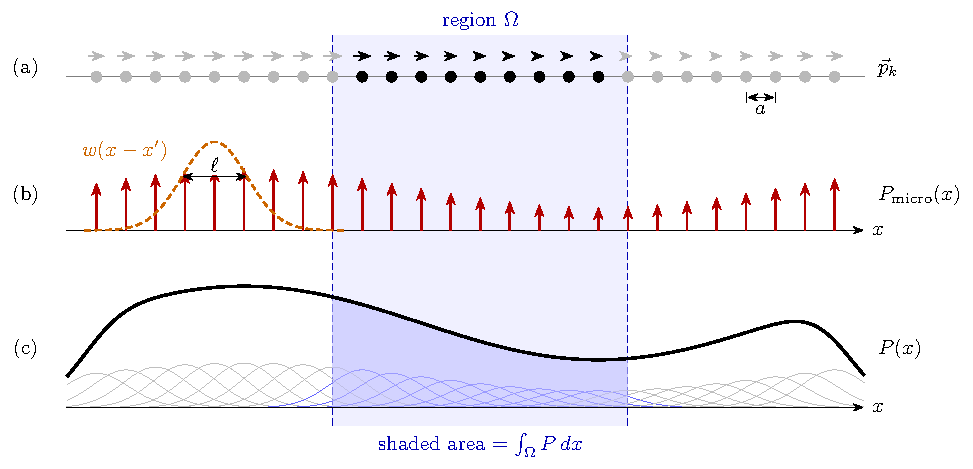
\includegraphics{figures/averaging.pdf}
\caption{Averaging of a one-dimensional chain of dipoles. (a)~Discrete dipoles $\vec p_k$ with interatomic distance $a$; dipoles inside $\Omega$ in black. (b)~Microscopic dipole density as delta peaks, with one averaging window $w$ of width $\ell \gg a$. (c)~Contributions $p_k\,w(x-x_k)$ of single dipoles (thin curves) and their sum, the smooth polarization $P(x)$ (thick curve). Dipoles far outside $\Omega$ (gray) do not contribute to the shaded area, and dipoles within $\ell$ of the boundary contribute partially.}
\label{fig:averaging}
\end{figure}

\paragraph{Limitation of the averaging picture in periodic crystals.}
The averaging assumes that the charge can be grouped into localized dipoles $\vec p_k$. In a periodic crystal, the electron density is continuous, so the dipole moment of a unit cell depends on how the cell is chosen. Different choices give bulk polarizations that differ by integer multiples of a \textcolor{blue}{polarization quantum}, which is proportional to a lattice vector divided by the cell volume. Only changes in $\vec P$, for example under strain or atomic displacement, are physical. The modern theory of polarization computes these changes from the Berry phase of the Bloch wave functions (King-Smith and Vanderbilt, 1993; Resta, 1994).

\paragraph{Electric field of a single dipole.}
The field of a volume of dipoles is built from the field of a single dipole. For a point dipole $\vec p$ at the origin, the dipole term of the multipole expansion gives the potential
\begin{equation*}
    \phi(\vec R) = \frac{\hat R\cdot\vec p}{R^2} = \frac{\vec p\cdot\vec R}{R^3}.
\end{equation*}
The electric field is the negative gradient of the potential, $\vec E = -\vec\nabla\phi$. With $\vec\nabla(\vec p\cdot\vec R) = \vec p$ and $\vec\nabla R^{-3} = -3\vec R/R^5$,
\begin{equation*}
    \vec E(\vec R) = -\frac{\vec p}{R^3} + \frac{3(\vec p\cdot\vec R)\,\vec R}{R^5}.
\end{equation*}
The field of a point dipole is therefore
\begin{equation}
    \boxed{
    \vec E(\vec R) = \frac{3(\vec p\cdot\hat R)\,\hat R - \vec p}{R^3}.
    }
\end{equation}

\paragraph{Potential of a volume of dipoles.}
Because $\vec P$ is a smooth density, the volume element $d^3r$ at the source point $\vec r$ carries the dipole moment $\vec P(\vec r)\,d^3r$. A dipole at $\vec r$ instead of the origin has the potential $\vec p\cdot(\vec R - \vec r)/|\vec R - \vec r|^3$. Summing the contributions of all volume elements of a material occupying $\Omega$ gives
\begin{equation*}
    \phi(\vec R) = \int_\Omega \frac{\vec P(\vec r)\cdot(\vec R - \vec r)}{|\vec R - \vec r|^3}\,d^3r.
\end{equation*}
\textcolor{red}{From now on, $\vec\nabla_{\vec r}$ denotes the gradient with respect to the source point $\vec r$, whereas $\vec\nabla$ without a subscript still acts on the field point $\vec R$.} The integrand simplifies with the identity
\begin{equation*}
    \vec\nabla_{\vec r}\,\frac{1}{|\vec R - \vec r|} = \frac{\vec R - \vec r}{|\vec R - \vec r|^3},
\end{equation*}
so that
\begin{equation*}
    \phi(\vec R) = \int_\Omega \vec P\cdot\vec\nabla_{\vec r}\,\frac{1}{|\vec R - \vec r|}\,d^3r.
\end{equation*}

\paragraph{Bound charges as the sources of the polarization potential.}
The product rule $\vec\nabla_{\vec r}\cdot(f\vec P) = f\,\vec\nabla_{\vec r}\cdot\vec P + \vec P\cdot\vec\nabla_{\vec r} f$ with $f = 1/|\vec R - \vec r|$ splits the integrand into two parts,
\begin{equation*}
    \phi(\vec R) = \int_\Omega \vec\nabla_{\vec r}\cdot\left(\frac{\vec P}{|\vec R - \vec r|}\right) d^3r
    - \int_\Omega \frac{\vec\nabla_{\vec r}\cdot\vec P}{|\vec R - \vec r|}\,d^3r.
\end{equation*}
The divergence theorem turns the first integral into an integral over the boundary $\partial\Omega$, with outward unit normal $\hat n$ and surface element $dS$. The potential of the polarized material is therefore
\begin{equation}
    \boxed{
    \begin{gathered}
    \phi(\vec R) = \oint_{\partial\Omega} \frac{\sigma_b(\vec r)}{|\vec R - \vec r|}\,dS
    + \int_\Omega \frac{\rho_b(\vec r)}{|\vec R - \vec r|}\,d^3r,\\[4pt]
    \sigma_b = \vec P\cdot\hat n, \qquad \rho_b = -\vec\nabla_{\vec r}\cdot\vec P,
    \end{gathered}
    }
\end{equation}
where $\sigma_b$ is the \textcolor{blue}{bound surface charge density} and $\rho_b$ is the \textcolor{blue}{bound volume charge density}. A polarized material thus produces the same potential as these two charge distributions. In particular, a uniform polarization has $\rho_b = 0$ and produces only a surface charge. Figure~\ref{fig:boundcharge} shows the origin of both bound charges in a chain of dipoles.

\begin{figure}[htbp]
\centering
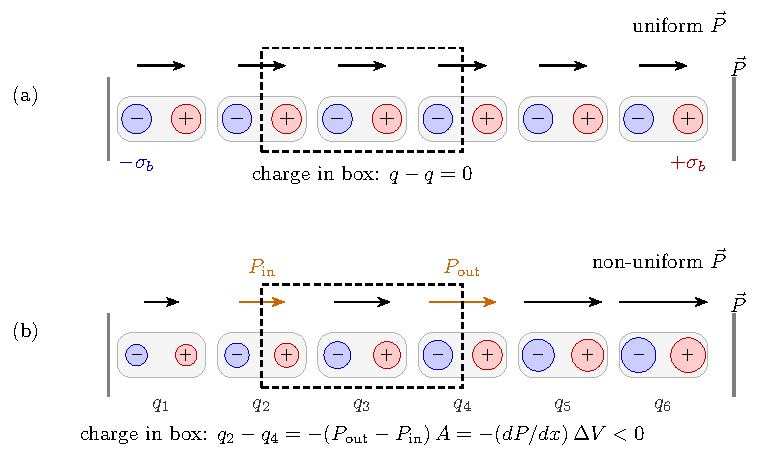
\includegraphics{figures/boundcharge.pdf}
\caption{Bound charges of a chain of dipoles between two surfaces. (a)~Uniform polarization: the charges of neighboring dipoles cancel inside the box, and only the surfaces carry the uncompensated charges $\pm\sigma_b$. (b)~Polarization increasing to the right: the box holds $+q_2$ and $-q_4$ with $q_4 > q_2$, so it carries the net charge $-(dP/dx)\,\Delta V$. Here $A$ is the cross-sectional area and $\Delta V$ the volume of the box.}
\label{fig:boundcharge}
\end{figure}
